\documentclass[a4paper,11pt]{article}

% ---- Paket ----
\usepackage[format=plain,font=normal]{caption}
\usepackage{lmodern}
\usepackage[T1]{fontenc}
\usepackage[letterspace=150]{microtype}
\usepackage{color}
\usepackage{lipsum,mathtools}
\usepackage[utf8]{inputenc}
\usepackage{geometry}

% För figurer och subfigurer
\usepackage{graphicx}
\usepackage{subcaption}

\usepackage{changepage}
\usepackage{placeins}
\usepackage{parskip}
\usepackage[english]{babel}
\usepackage{float}
\usepackage{booktabs}
\usepackage{enumitem}
\usepackage{amsmath}
\usepackage{blindtext}
\usepackage{scrextend}
\usepackage[normalem]{ulem}
\usepackage{float}
\useunder{\uline}{\ul}{}
\usepackage{titlesec}
\usepackage{amsmath}
\usepackage{amssymb}
\usepackage[export]{adjustbox}
\usepackage[style=ieee]{biblatex}
\usepackage{url}
\usepackage{csquotes}
\usepackage{dirtytalk}
\usepackage{comment}
\usepackage{fancyhdr}

% ---- Inställningar ----
\setlength{\parskip}{1em}   % whitespace between paragraphs
\setlength{\parindent}{0em} % no indentation in new paragraphs
\numberwithin{equation}{section}
\newcommand\tab[1][0.5cm]{\hspace*{#1}}
\addbibresource{references.bib}
\graphicspath{{images/}}
\lhead
\rhead
\pagestyle{fancyplain}

% ---- Färger ---
\definecolor{light-gray}{gray}{0.40}
\definecolor{mygreen}{RGB}{28,172,0}
\definecolor{mylilas}{RGB}{170,55,241}

\begin{document}
%\begin{comment}

\thispagestyle{empty}
\begin{titlepage}
    \centering
    \vfill\vfill
    \Huge A Unity Extension for Procedurally Generating Cities
    \noindent\makebox[\linewidth]{\textcolor{light-gray}{\rule{\paperwidth}{0.1pt}}}
    \begin{center}
        \LARGE{Group 85} \\ [0.3cm]
        \large	
        \begin{minipage}[t]{0.48\textwidth}
            \begin{flushright}
                Alma Eriksson \\ [0.3cm]
                David Hultsten \\ [0.3cm]
                Ludvig Liljeqvist \\ [0.3cm]
            \end{flushright}
        \end{minipage}%
        \hfill{\color{light-gray}\vline}\hfill
        \begin{minipage}[t]{0.48\textwidth}
            \begin{flushleft}
            David Hall \\ [0.3cm]
            William Johnsson \\ [0.3cm]
            Ludwig Lundholm Hultqvist \\ [0.3cm]
            \end{flushleft}
        \end{minipage}
    \end{center} 
    \large{\today}
    \vfill
\end{titlepage}
\clearpage
%\end{comment}

\begin{comment}

\begin{titlepage}
\thispagestyle{empty}
\title{ \Huge{A Tool for Procedurally Generated Cities in Games} \noindent\makebox[\linewidth]{\textcolor{light-gray}{\rule{\paperwidth}{0.1pt}}}}
\author{\LARGE{Group 85} \\\\ 
[0.30cm] Alma Eriksson, David Hall,\\
[0.30cm] David Hultsten, William Johnsson,\\
[0.30cm] Ludvig Liljeqvist, Ludwig Lundholm Hultqvist
\\[0.1cm]}
\maketitle
\thispagestyle{empty}
\end{titlepage}
\clearpage
\maketitle

\end{comment}

\setcounter{page}{0}
\thispagestyle{empty}
\tableofcontents
\pagebreak
\section{Background}%sammanfattnign om unity och PCG 
Since the introduction of the first video games, the gaming industry has been booming with innovations of consoles and creating content. An availability of public game development platforms, such as Unity, has also opened the doors for private game developers to enter this market as well. However, improvements in computational power has created a demand of graphical applications containing more detail and realism, to a point were the gaming industry had to utilize new concepts to meet this demand. One way of providing such graphical applications is through using \textit{procedural content generation}, or simply \textit{PCG}. 

The concept has been utilized throughout many popular games, such as \textit{Minecraft} and \textit{Diablo} as two honorable mentions. Since PCG is relatively complicated and hard to comprehend, private game developers may not be able to utilize it. Thus, to make it simpler for game developers to take part of this concept, this thesis presents how procedural content generation can be utilized in a Unity extension.


\subsection{Procedural Content Generation}
Procedural content generation, or PCG, can be defined as \say{the algorithmic creation of game content with limited or indirect user input.} \cite[p. 1]{shaker2016procedural} This means that PCG can be used to either create content fully automatically or with a low degree of human assistance.

Togelius et al present four arguments for using PCG \cite[pp. 141-142]{search-based_pcg}:
\begin{enumerate}
    \item PCG is memory efficient since content only has to be generated when it is needed.
    \item Using PCG is relatively effortless in terms of development time and expenses.
    \item PCG has a potential for being used to generate whole games of new kinds and with unlimited replayability.
    \item PCG can be used as a tool to make us humans think "out of the box" since it can provide us with content we probably would not have come up with on our own.
\end{enumerate}
 
Another reason for game developers to use PCG methods is that the algorithms are capable of creating vast amounts of game assets at a faster rate than 3D-artists. This will result in a potential cost reduction for the production, as entire teams will not be needed to work on this particular aspect of the game. On top of this, the algorithms can be designed in a way that the world is generated in real-time, creating an endless world for the player to explore. However, special care must be taken when writing PCG algorithms to create visually interesting and diverse worlds that does not break gameplay.

Procedural content generation may also be used as a complementary tool for worlds built manually. When utilized in this fashion, PCG does not generate new assets, but rather hides and reveals existing ones on demand. This is a necessary tool in games with larger worlds. In such worlds, objects need to be viewed at differing levels of detail, depending on distance to the player. When far away, many objects fit on the player's screen. Rendering them all in full detail can be detrimental to performance, and also unnecessary because of restraints on screen resolution. With the help of PCG, smaller assets can be hidden when viewed from a great distance, and the detail of larger ones can be downscaled. \cite[p. 57]{shaker2016procedural}

It is important to note that PCG is also used outside of the gaming industry. Two examples of this are SpeedTree~\cite{SpeedTree}, a tool for generating virtual foliage that is used by architects and animators and Esri CityEngine~\cite{CityEngine}, modeling software for creating immersive urban environments based on geographical data.

\subsection{Unity Editor extensions}
The Unity editor can be extended in order to improve the workflow for developers. There are several extension examples, many of which are available in the Unity Asset Store. A few examples of editor extensions are: \textit{ProBuilder}, \textit{Playmaker} and \textit{Shader Forge} \cite{unity-probuilder, unity-hutong-playmaker, unity-shadow-forge}. All of these examples have custom graphical interfaces, adding new functionality to the Unity editor.

\subsubsection{ProBuilder}
\textit{ProBuilder} is a Unity tool that can be used to design levels and create 3D models. The extension has been an optional addition to the official Unity editor since the 2018.1 version. Examples of games utilizing the tool are \textit{SUPERHOT} and \textit{Tunic} \cite{unity-probuilder}.

\begin{figure}[H]
    \centering
    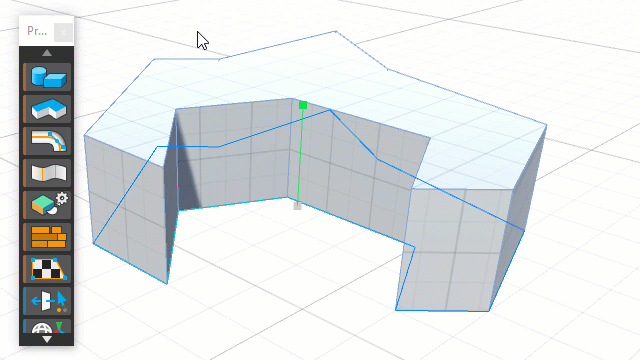
\includegraphics[width = 0.6\textwidth]{Planning report/images/probuilder-example.png}
    \caption{An example of the graphical interface of \textit{ProBuilder} \cite{unity-probuilder-procore}.}
    \label{fig:probuilder-editor}
\end{figure}

\begin{figure}[H]
\centering
\begin{subfigure}{.48\linewidth}
  \centering
  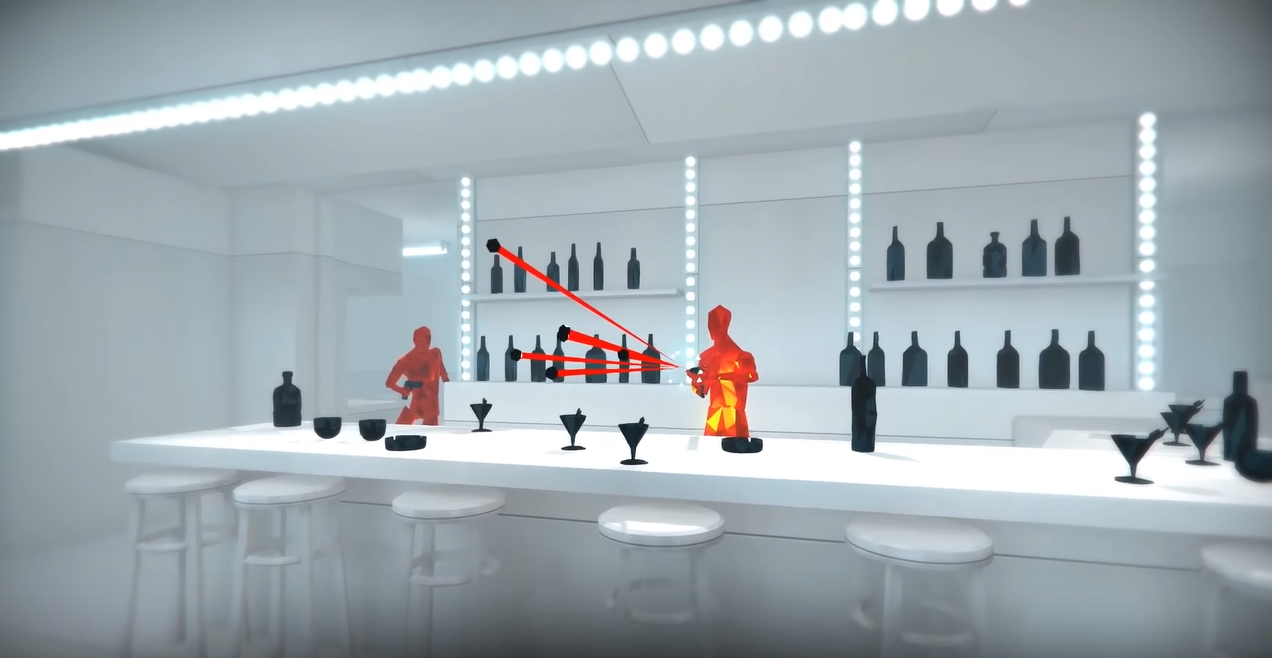
\includegraphics[width=1\linewidth]{Planning report/images/superhot-game.png}
  \caption{\textit{SUPERHOT}}
  \label{fig:superhot-game}
\end{subfigure}
~
\begin{subfigure}{.48\linewidth}
 \centering
  
\includegraphics[width=1\linewidth]{Planning report/images/tunic-game.png}
  \caption{\textit{Tunic}}
  \label{fig:tunic-game}
\end{subfigure}
\caption{Screenshots of two games developed with \textit{ProBuilder}.}
\label{fig:probuilder-games}
\end{figure}

\subsubsection{Playmaker}
\textit{Playmaker} is a visual scripting tool and has the highest rating in the Unity Asset Store. It is a tool for creating behaviours in games without writing code. Behaviours are instead defined with state machines in a custom graphical interface in Unity. Two examples of games that utilize the tool are: \textit{Hearthstone} and \textit{Hollow Knight} \cite{unity-hutong-playmaker}.

\begin{figure}[H]
    \centering
    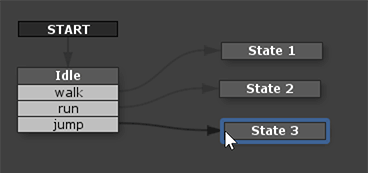
\includegraphics[width = 0.6\textwidth]{Planning report/images/playmaker-example.png}
    \caption{Screenshot of the graphical interface of \textit{Playmaker}.}
    \label{fig:playmaker-editor}
\end{figure}

\begin{figure}[H]
\centering
\begin{subfigure}{.48\linewidth}
  \centering
  
\includegraphics[width=1\linewidth]{Planning report/images/hearthstone-game.png}
  \caption{\textit{Hearthstone}}
  \label{fig:hearthstone-game}
\end{subfigure}
~
\begin{subfigure}{.48\linewidth}
  \centering
  
\includegraphics[width=1\linewidth]{Planning report/images/hollow_knight-game.png}
  \caption{\textit{Hollow Knight}}
  \label{fig:hollow-knight-game}
\end{subfigure}
\caption{Screenshots of two games developed with \textit{Playmaker}.}
\label{fig:playmaker-games}
\end{figure}

\subsubsection{Shader Forge}
\textit{Shader Forge} was released to the Unity Asset Store in 2011 \cite{unity-shadow-forge-forum} but has since then been removed. It is, however, still available on GitHub as an open-source repository \cite{unity-shadow-forge-github}. It is a tool for creating shaders without writing any code and has its own custom graphical interface based on nodes. The tool has been promoted by game developers known for games such as \textit{Dear Esther} and \textit{Knytt Underground} \cite{unity-shadow-forge}.

\begin{figure}[H]
    \centering
    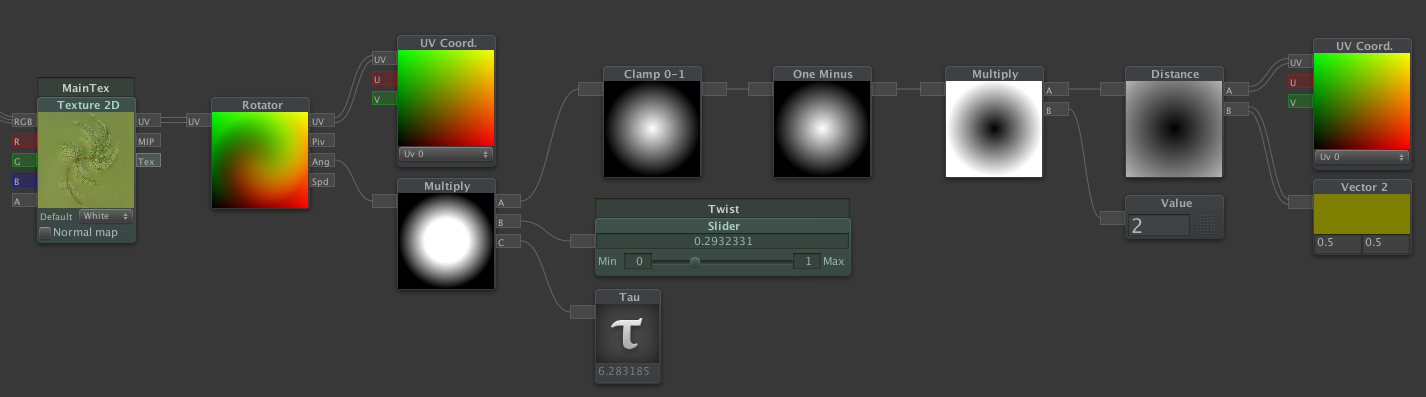
\includegraphics[width = \textwidth]{Planning report/images/unity-shader-forge.jpg}
    \caption{A screenshot of the graphical interface of \textit{Shader Forge} \cite{unity-shadow-forge-forum}.}
    \label{fig:shader-forge-editor}
\end{figure}
\newpage
\section{Games using Procedural Content Generation}
Procedural content generation is, as described previously, a powerful tool for generating content in games in ways that might not be possible to be created manually. PCG, however, is a broad concept and is utilized i many games i various ways. How a few of the more popular games utilizes PCG is described in this section. 

\subsection{Diablo}
\textit{Diablo} is a fantasy game about a group of warriors on a mission to hunt down the demon lord Diablo, who is threatening the village of Tristram. To reach Diablo in Hell, the player must go through a series of request that takes them on a journey through the difficult dungeon. \textit{Diablo} was likely a success because of its early on uses of PCG algorithms that randomly created dungeons for each new level. The developers used what they called a "Dynamic Random Level Generator" to generate a new dungeon for each level \cite{Diablo_PCG}. The generator provided a new gaming experience for the player every time the game was played. 

\begin{figure}[H]
    \centering
    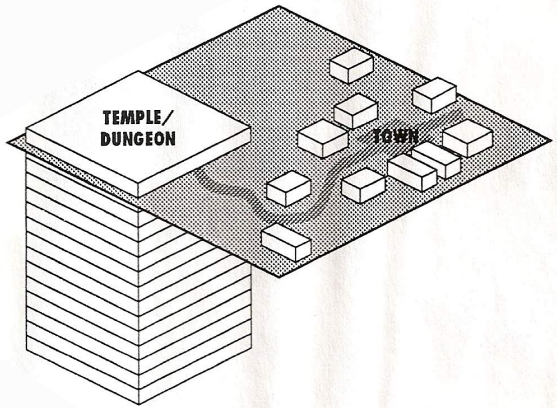
\includegraphics[width=0.5\linewidth]{Planning report/images/diablo.jpg}
    \caption{Level structure plan from the \textit{Diablo} pitch, the year 1994.}
    \label{fig:diablo_plan}
\end{figure}{}


\subsection{Minecraft}
\textit{Minecraft} is a popular game with a three-dimensional world consisting of cubes of earth, wood and other materials. The game is multi-functional, meaning that players can decide if they want to build structures and obtain objects from the world. There are environmental hazards that can kill players' avatars, but it is possible to avoid these in the game. \textit{Minecraft} is based on algorithms like Perlin Noise to generate unique terrains with large voxels~\cite{minecraft_PCG}. The game also uses Whittaker diagrams to determine what plants and other terrain features that should be added in different biomes. This makes the world more realistic, as seen in figure \ref{fig:biome}. As of May 2019, 10 years since its official release, \textit{Minecraft} has sold over 176 million copies~\cite{Minecraft_10ys}, proving its huge success.

\begin{figure}[H]
\centering
\begin{subfigure}{.48\linewidth}
  \centering
  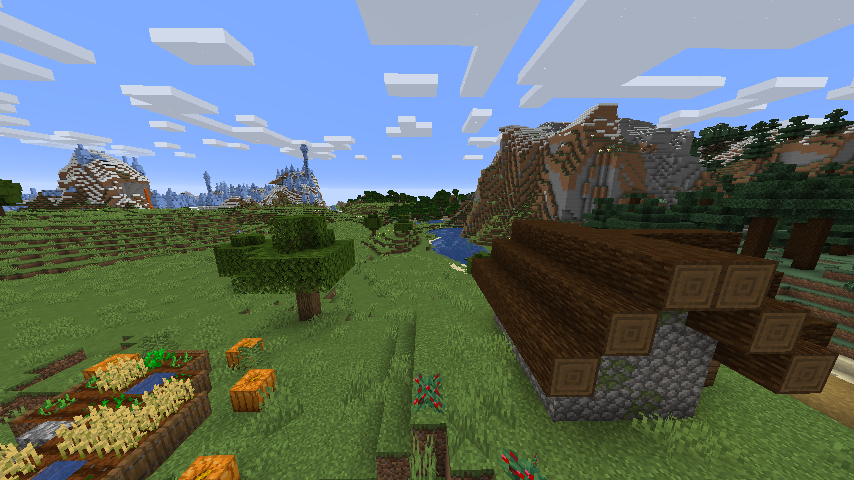
\includegraphics[width=1\linewidth]{Planning report/images/minecraft1.png}
  \caption{Minecraft world}
  \label{fig:minecraft}
\end{subfigure}
~
\begin{subfigure}{.48\linewidth}
  \centering
  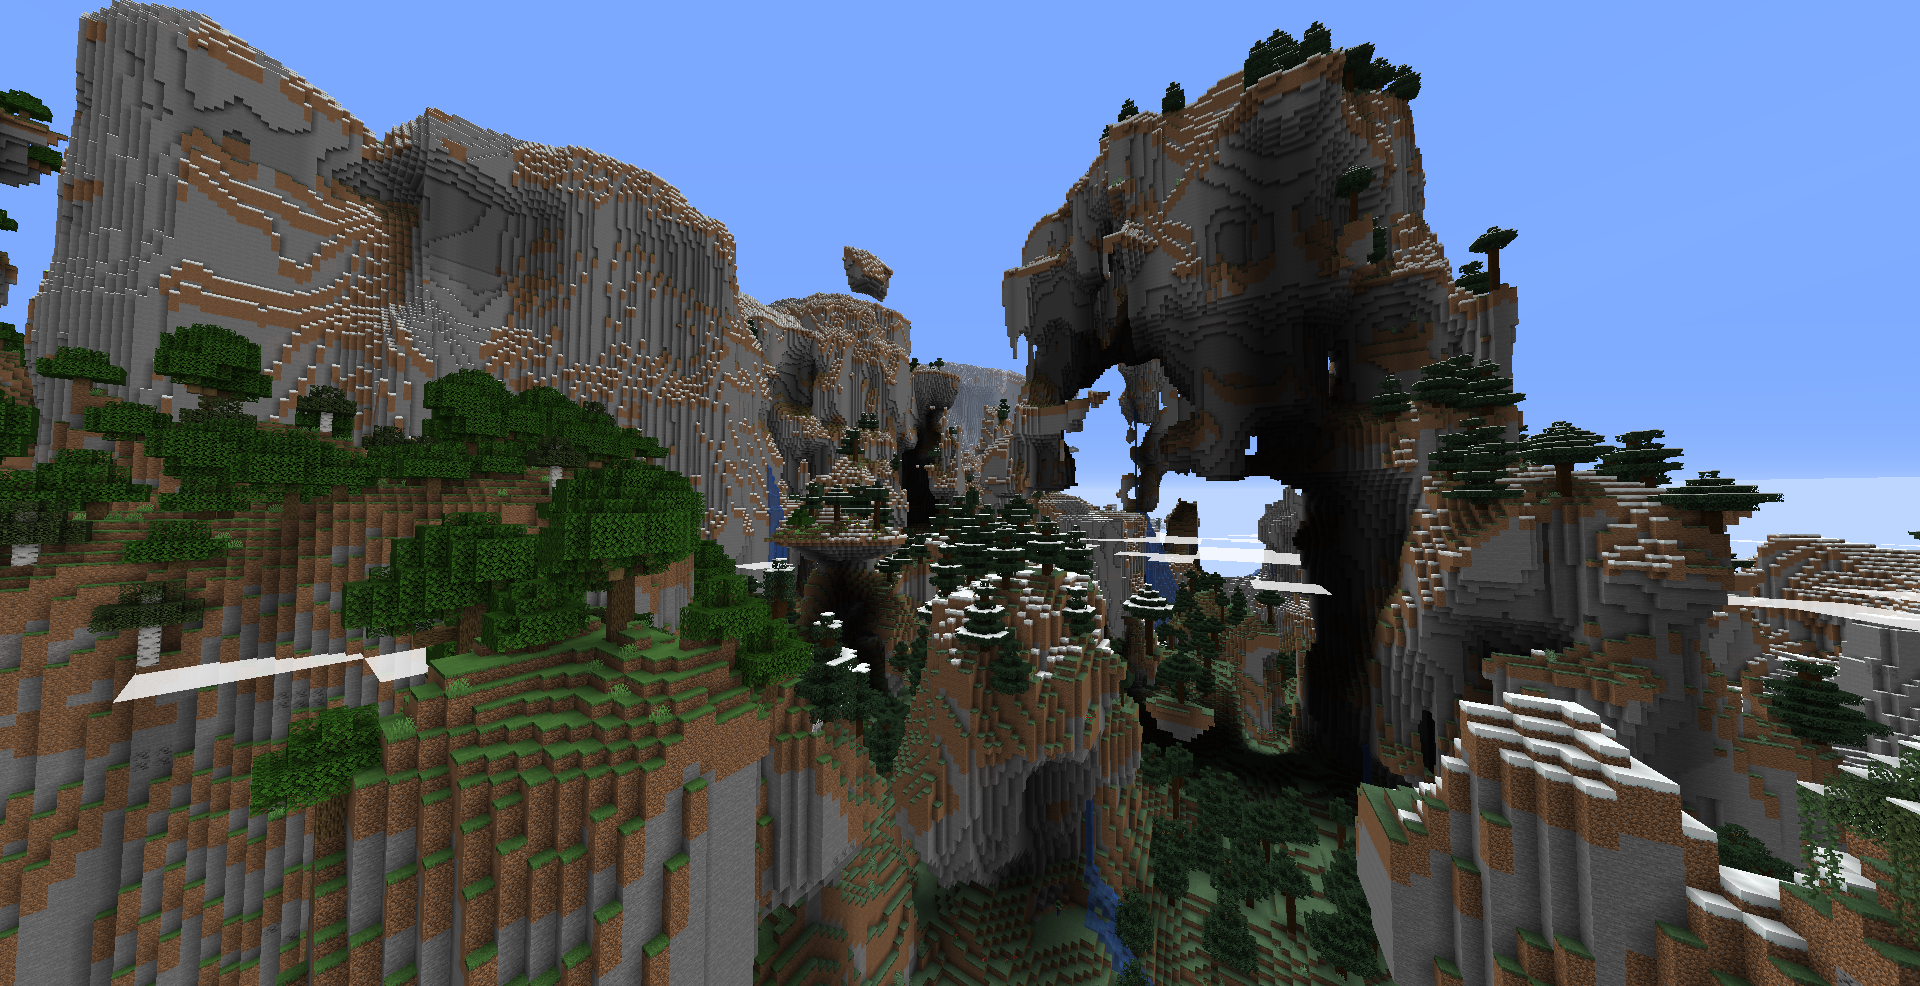
\includegraphics[width=1\linewidth]{Planning report/images/minecraft2.png}
  \caption{Amplified world in Minecraft}
\end{subfigure}
\caption{Screenshots of Minecraft.}
\label{fig:2_minecraft}
\end{figure}

\begin{figure}[H]
    \centering
    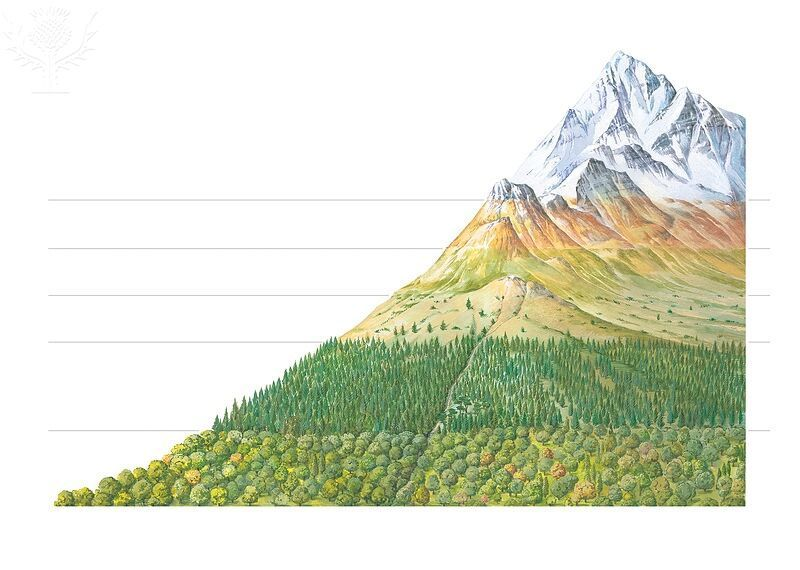
\includegraphics[width=0.5\linewidth]{Planning report/images/biome.jpg}
    \caption{Biome and vegetation altitude zones}
    \label{fig:biome}
\end{figure}


%It is a valid theory that the random generation of worlds using PCG has something to do with the game's overwhelming success.


%Take for example the popular game Minecraft [32], where players find themselves in a world made of three-dimensional cubes of earth, wood, lava and other materials. First steps usually include punching at a tree to obtain some wood, which is then used to build tools to mine other blocks. While it is technically possible to beat the game by defeating an end boss, most players entertain themselves with building structures and obtaining stuff from the world. There are enemies in the game, and other environmental hazards that can kill the player’s avatar, but it is possible to largely avoid violence and focus on building interesting structures


%A few examples of games using PCG are \textit{Diablo} for generating maps, \textit{Spore} for creature animations and \textit{Minecraft} for landscapes and caves \cite[p. 5]{shaker2016procedural}. Perhaps the greatest example of a game utilizing PCG is \textit{No Man's Sky}, which procedurally generates everything from vegetation and creatures to landscapes and planets and thus creates a virtually endless and unique universe for its players to explore \cite{MIT_No_Mans_Sky}.

%As of May 2019 and after 10 years of its official release, \textit{Minecraft} has sold over 176 million copies \cite{Minecraft_10ys}. It is a valid theory that the random generation of worlds using PCG has something to do with the game's overwhelming success.


% skriva mer om grids och cul de sac 

% hur pcg används i andra syften än spel
\newpage
\section{Purpose}
The focus of this thesis is to investigate how game development can be made less time-consuming and more cost-effective, by developing a tool for creating 3D cities and surrounding terrain using procedural content generation. Cities developed with the tool are supposed to be usable in a variety of city-based games to make development processes more effortless.

\begin{comment}
The focus of this theses is on the algorithms for Procedural Content Generation; more specifically, a tool for automating the creation of realistic cities to make game development cost-effective and less time-consuming.
\end{comment}

\section{Goal}
The primary goal is to provide a useful and interactive tool for game developers to design cities and surrounding terrains in real-time. Firstly, the tool should be able to generate terrain with elements such as mountains, rivers and lakes that depend on certain probability parameters. The developer should then be able to mark an area where a city should be placed. Through the use of procedural algorithms, a city with, for instance, roads, houses and skyscrapers shall be placed on the terrain. This requires relatively fast algorithms, since it would be frustrating having to wait for the generation to complete.

Another goal is to make the generated cities open for customization, in terms of changing graphical elements, adding functionality or other types of assets. This is important since game developers using the tool should be able to create any city-based game imaginable. The tool should preferably not hinder the creativity of its users.

There are also various other elements that could be added to the tool, for instance simulated humans that are walking or driving cars. Such ideas will, however, have to wait until the earlier mentioned goals of this project have been achieved.

At last, the platform should also provide insights about using PCG in games, to provide a knowledge base for game developers wanting to implement such algorithms in their own designs. This means that different algorithms for generating cities and terrain shall be studied, to discuss their advantages and disadvantages.
\newpage
\section{Delimitations}
\label{section:delimitations}

To better utilize procedural content generation as a tool for creating custom worlds in games, this study is solely focused on developing a tool for game development and not on creating actual gameplay. The user will only be able to use it to generate the layout and contents of the world.

The tool will be developed to allow developers to use it for developing most types of games. As of now, it will not be focused on specific game genres, to give the tool a wide range of use cases. This may however change further on, due to the time constraints of the project and possible constraints of the PCG algorithms.

The generated content will mainly be based on credible aesthetics and not on realistic functionality. Cities, for instance, will be generated to have realistic appearance, but will lack behaviors of a real life city such as working freeways, subways and sewage systems. They will also not be realistically accurate of how real cities were built and grew larger. To focus on credibility rather than realism is mainly due to the time constraints of this project. To accurately mimic reality would require a lot of time spent on, for instance, historical research of cities. This was therefore left out of the project. By not generating a too realistic world, we ensure that we don't limit room for creativity for users of the tool.

Visual fidelity is not a priority for the generated content. The focus of the thesis is instead to spend more time developing the algorithms for procedural content generation of major city components rather than drawing sophisticated art assets. This also leaves room for developers to apply their own textures to the generated city and terrain.
\newpage
\section{Methodology}
\label{section:methodology}

As this project requires a good understanding of concepts for procedural content generation and various implementations of it, the initial objectives are to conduct research on the subject before starting on the actual implementation. The research mainly includes finding commonly used algorithms, some of which are described in section \ref{section:theory}, as well as how they are implemented and used in various games and other cases. Further on, the algorithms are then evaluated on their suitability to generate various aspects of realistic city environments. The best candidates are then to be selected for different cases, after which implementation of them can begin. Finer details, such as intersection handling for road and other potential problems, are algorithm-dependent and are to be handled further on in the project. 

The tools to be used throughout the project and how the work is to be organized is described below.

\subsection{Development tools}
Various tools and platforms can be used for the creation of a game development tool. Since the main focus of this project is to develop the PCG algorithms used by the tool, and not the creation of a game engine, the tool will be built using the Unity platform \cite{Unity}. Most of the project members do not possess a lot of game development experience and Unity did not seem to have a steep learning curve, which is why it was chosen for the project.

As a result of the close integration between Unity and the C\# programming language, this is the language which the PCG tool is to be developed in. On top of this, C\# is a type of language that all project members had previous experience working with. To also be able to create 3D assets that are not created directly by the tool, the Blender tool will be used as well \cite{Blender}. However, since the main focus is to develop a PCG tool and not 3D assets, Blender may not be used for the final product.

\subsection{Agile development}
There are many different approaches of developing and managing a software project. Because of uncertainties about the final feature specifications of the developed tool, an iterative approach was deemed necessary, and linear approaches such as the waterfall methodology was to be avoided \cite{Waterfall}. In order to work in an agile way, the objectives of the project have to be organized into relatively short time periods. It is also important to parallelize the development between project members, which is why the project will be developed by following a, perhaps simpler, version of the agile methodology called "Scrum" \cite{Scrum}. Due to its suitability with iterative processes and prior experiences from several project members, this was deemed the most reasonable approach.

In this methodology, the project is divided into "sprints", consisting of an agreed time-span of approximately two weeks. However, due to external factors such as exam weeks and longer periods of self studies, the time-span of some sprints have been adjusted to three weeks instead. How the sprints are preliminary scheduled is displayed in section \ref{fig:timetable}.

Each sprint will start with a planning meeting, consisting of scoping the sprint and dividing tasks among the project members. During sprints, the project members will meet one or a few additional times depending on the length of the sprint, to synchronize the progress. The sprints end with a meeting consisting of a sprint review and a retrospective, to review the outcome of the sprint, as well as to reflect on the sprint in general.
\newpage
\section{Theory}
\label{section:theory}
This section covers the theory behind different aspects of the city generation tool of this thesis, namely: PCG approaches and methods for generating certain city elements as well as the surrounding terrain and a few words about developing extensions for Unity.

\subsection{Constructive and Generate-And-Test approaches to PCG}
The difference between constructive algorithms for PCG and generate-and-test algorithms is that the former only involves the actual generation of the content; once the content has been generated, the process is done. The latter, however, also involves testing the content and making sure that it meets all specified requirements. If it does not, it is ignored and the process starts over and repeats until all criteria are met \cite{search-based_pcg}.

\subsection{The Search-based approach to PCG}
The search-based approach to PCG is based on the previously mentioned approach called "generate-and-test". The difference is that generated content in the search-based approach is graded for its quality, unlike generate-and-test, where it is instantly discarded if not optimal. The grading is done with fitness functions (also called evaluation functions) that determine how suitable the content is in the context. The generation of content depends on previous results and fitness scores to increase the content quality \cite{search-based_pcg}. The search-based approach consists of three main parts: the search algorithm, the content representations and the evaluation functions \cite[pp. 17-20]{shaker2016procedural}.

\subsubsection{Content representations}
Content representations can be interpreted as blueprints, defining how different types of content are to be generated \cite[p. 18]{shaker2016procedural}. A game level, for instance, probably has to contain certain elements to fit into the game that is being developed. The content representation can therefore contain data about what is required and can then be used to generate actual levels. 

Togelius and Shaker describe content representations in the terms of "genotypes" and "phenotypes" in the context of evolutionary search algorithms. The former is what is used to generate content and the latter is the actual generated content, derived from the genotype \cite[pp. 18, 20]{shaker2016procedural}. Referencing the earlier example about game levels; the genotype would be the data about what is required in the level and the phenotype would be the generated level itself.

\subsubsection{Evaluation functions}
Evaluation functions determine how well-generated content fits into the context. An example of this is a game level that has been generated and then evaluated to verify that it is possible to beat and that it is neither too easy nor hard to play. There are at least three types of evaluation functions: direct, simulation-based and interactive \cite[pp. 18-24]{shaker2016procedural}.

% Direct
Evaluation functions that directly calculate fitness values based on the generated content's attributes are called "direct". Such functions can either be driven by theory or by data. The former means that the evaluation is based on theories about how players will experience the content. The latter means that the evaluation is based on collected data and statistics about player experience \cite[p. 23]{shaker2016procedural}.

% Simulation-based
As the name suggests, simulation-based evaluation functions involve simulating the use of generated content to evaluate their respective fitness values. The simulation is done by utilizing AI agents that for example play a generated game level to make estimations. Agents can either be dynamic or static, meaning that they either adapt during the simulation or not \cite[pp. 23-24]{shaker2016procedural}.

% Interactive
Evaluation functions can also be based on human interaction, meaning that human actions can determine the fitness of generated content. An example is giving different fitness values to generated weapons in games, depending on how much they are used by actual human players \cite[p. 24]{shaker2016procedural}.

\subsubsection{Search Algorithms}
There are different types of search algorithms, such as: Evolutionary, exhaustive, random and solver-based. Togelius and Shaker describes an evolutionary search algorithm where the number of generation surviving ''individuals'' (content) is represented by $\mu$ and where the number of ''offspring'', derived from the previous generation, is represented by $\lambda$. The sum of these variables is the total size of the content population when generating. The algorithm consists of eight steps, where only the second one is optional \cite[p. 18-20]{shaker2016procedural}:

\begin{enumerate}
    % Step 1: Initialization
    \item A population with the size of $\mu + \lambda$ has to be initialized in order to generate anything. Since this is the initialization step and is only executed once at the very start of the algorithm, this can be done in any way that is deemed appropriate in the context. The initial population can for example consist of individuals that are man-made, from earlier uses of the algorithm or generated at random.
    % Step 2: Shuffle the population (start of a generation)
    \item Optionally shuffle the population in order to avoid loss-of-gradient situations \cite{shaker2016procedural}, meaning that some subpopulations otherwise could start dominating others \cite{Spatial-Embedding-and-Loss-of-Gradient}.
    % Step 3: Evaluate individuals
    \item The fitness for each individual content is calculated to a numeric value by using it as a parameter in an evaluation function.
    % Step 4: Sort by fitness
    \item The whole population is sorted by the fitness in an ascending order.
    % Step 5: Discard bad individuals
    \item Since $\mu$ is the number of surviving individuals after a generation, a total of $\lambda$ individuals has to be discarded. The ones getting ''killed'' have the worst fitness scores of the population and are therefore not fit to generate any offspring for the next generation.
    % Step 6: Replace the discarded individuals with copies of good ones
    \item The discarded individuals are replaced by copies of the ones with higher fitness scores. Depending on the proportions between $\mu$ and $\lambda$, some elite individuals might not get copied at all or might be copied several times in order to reach the number of $\lambda$ copies, i.e., the population size does not change.
    % Step 7: Mutate some individuals
    \item A number of $\lambda$ individuals are randomly chosen to be mutated (modified) in arbitrary ways. An example of a mutation type is Gaussian mutation.
    % Step 8: Choose to stop or to continue
    \item Depending on if an individual is deemed good enough, based on its fitness score, the algorithm is stopped. It is also stopped if the number of executed iterations is equal to a specified maximum. The algorithm otherwise repeats everything from the second step and thus starts a new generation of individuals.
\end{enumerate}

\subsection{Terrain generation}
A common feature in games is varying terrain which is used to create interesting worlds to explore or sometimes being an integral part of the gameplay.

\subsubsection {Noise functions}
For generating terrain features such as heights, the most common approach is to generate an intensity map represented by a 2D matrix containing the brightness of each pixel \cite[pp. 58-59]{shaker2016procedural}. This can then be used to determine the different heights of the terrain through displacement mapping. An initial attempt at creating such a map could be to assign random values in the matrix as displayed in figure \ref{fig:random-noise} but in the case of terrain this would look like random spikes which would not be suitable for a game environment. To combat this, a type of gradient noise can be used, which was formally described by Ken Perlin in 1985~\cite{image-synthesizer} to generate more realistic looking textures compared to what was available at the time. This method was later improved by Perlin in 2001 where he introduced "simplex noise"~\cite{improving-noise} as seen in figure~\ref{fig:simplex-noise}. Compared to classic Perlin noise this improved algorithm scales to higher dimensions with less computational overhead and is easier to implement in hardware. 

To generate simplex noise in two dimensions, space is divided into simplexes (triangles in this case), where pseudo-random gradients are placed at the corner of each simplex. For every point in the space, the contribution of each simplex is calculated based on the \say{multiplication of the extrapolation of the gradient ramp and a radially symmetric attenuation function.}~\cite{simplex-demystified}.

The issue of using noise functions is that every location is independent of the others, which might make it feel like there is not enough uniqueness for a game environment. Multiple noise maps, controlling different aspects of the terrain, can, however, be used together to create, for example, overhangs and caves, thus making the terrain more interesting.

\begin{figure}[H]
\centering
\begin{subfigure}{.3\linewidth}
  \centering
  
\includegraphics[width=1\linewidth]{random-noise.png}
  \caption{Random noise}
  \label{fig:random-noise}
\end{subfigure}
~
\begin{subfigure}{.3\linewidth}
  \centering
  
\includegraphics[width=1\linewidth]{simplex-noise.png}
  \caption{Simplex noise}
  \label{fig:simplex-noise}
\end{subfigure}
\caption{Two types of noise}
\end{figure}

\subsubsection{Using Agents}
While the inherent randomness of PCG methods like Perlin noise is what makes them desirable, it can often be to the detriment of customizability. Designers can tailor their terrain to some degree, but only on a global level through the adjustment of a set of parameters. Agent-based terrain generation is an alternative which retains customizability while also providing features expected of PCG, such as randomness, unpredictability, speed, and so on \cite[64]{shaker2016procedural}.

Professors Jonathon Doran and Ian Parberry from The University of North Texas describe a way of procedurally generating terrain through software agents \cite{agentbasedTerrain}. Their method is based on five different types of agents. These agents work concurrently to simulate natural phenomena by sensing their environment and changing it at will. Designers can influence the generation of terrain by adjusting the number of agents of each type, or by changing their lifespan by restricting the number of actions they can perform. Once the maximum number of actions is reached, the agent becomes inactive.

Agents can modify the environment by performing three main tasks:

\begin{itemize}
    \item Coastline: The first phase in which multiple agents generate the main shape of the terrain.
    \item Landform: In the next phase more agents are employed to generate the more detailed features of the land. These include lowlands, beaches, and the details of mountains. The agents work simultaneously.
    \item Erosion: In the last phase, pieces of the terrain are chipped away to create rivers. The number of rivers depends on the number of agents.
\end{itemize}
Each phase contains several different types of agents; these include, but are not limited to: coastline agents, smoothing agents and beach agents. The coastline agents generate the rough parts of the environment, while the smoothing agents eliminate any resulting rapid elevation changes. After smoothing, beach agents traverse the shoreline, creating sandy areas near bodies of water.

\begin{figure}[H]
    \centering
    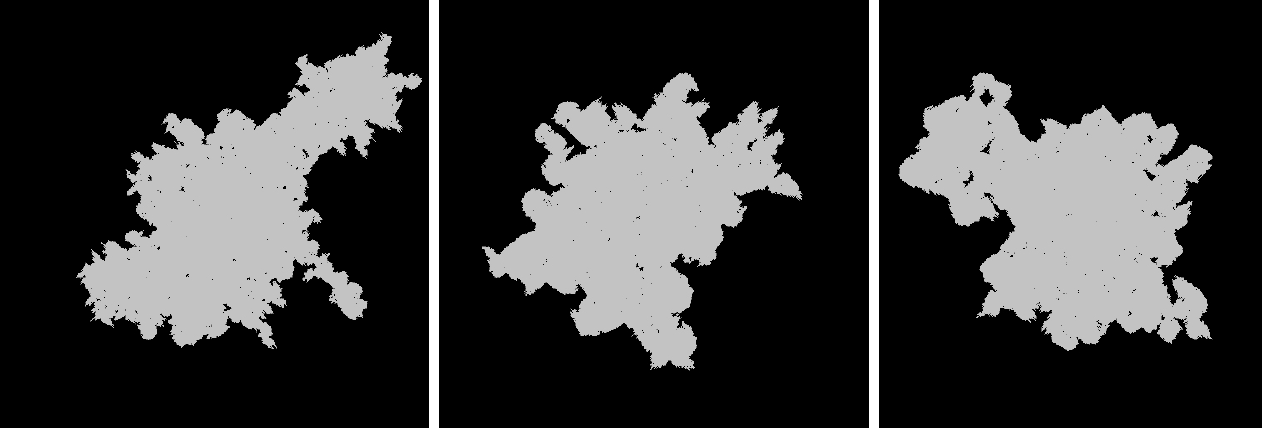
\includegraphics[width = 1\linewidth]{Planning report/images/coastline.PNG}
    \caption{Coastline generated by coastline agents with small, medium and large action sizes.}
    \label{fig:coastline}
\end{figure}
\begin{figure}[H]
    \centering
    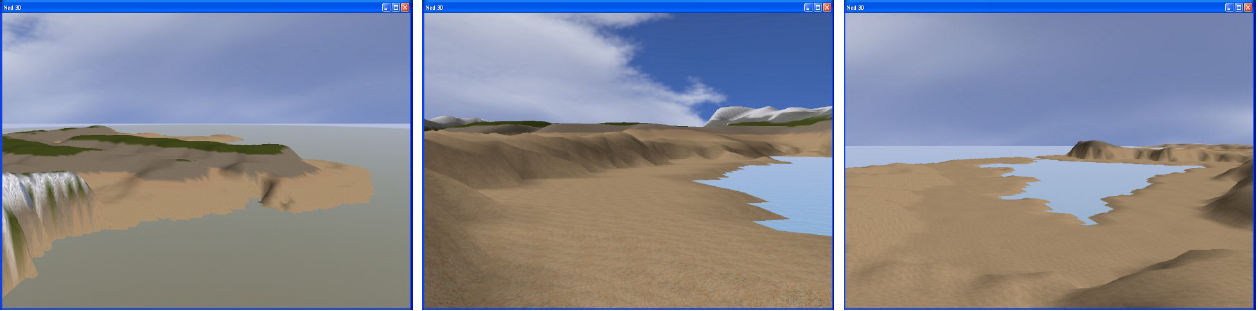
\includegraphics[width = 1\linewidth]{Planning report/images/beach.PNG}
    \caption{Beaches produced by beach agents with small, medium and large beach widths.}
    \label{fig:beach}
\end{figure}

By defining the agents and their sets of parameters, the generation of terrain can be suited to one's needs, and also remain unpredictable through the use of random seed numbers.

\subsection{Road generation}
This section will discuss different algorithms as related to the generation of road networks in a city environment.

\subsubsection{L-systems}
An early candidate for generating road networks was Lindenmayer Systems. L-systems are a special case of generative grammars and are typically used to generate visualizations of vegetation. Though they were introduced to model natural structures, they have also been used in city generation algorithms \cite{yoav-pascal}. 

% Grammars
Grammars are a set of symbols with rewrite rules that replace each symbol in the string with whatever symbols that rule dictates. The string of a grammar consists of terminals, non-terminals and an axiom, which is the initial string. A grammar may also associate parameters with rewriting rules, to modify certain properties of the result \cite{graphical_l-systems}. Rules in a non-deterministic grammar may either decide randomly which valid replacement should occur or use the parameters to determine which rule is the best fit, while deterministic ones only have a single derivation \cite[p. 75]{shaker2016procedural}. 

% L-systems
A defining feature of L-systems is that they rewrite the symbols in a given string in parallel each iteration. L-systems are not limited to the strict representation of strings; graphs and other objects may be represented by an L-system as well \cite[p. 75-79]{shaker2016procedural}. A grammar such as an L-system will generally consist of two parts when used for procedural modelling: the rewriting algorithm and an interpretation \cite{graphical_l-systems}. The interpreter is what will build a graphical representation of the generated data (such as vertices), and thus produce the model itself.

A simple, deterministic L-system: \\*
\begin{align*}
    &Rules: \\
    &\qquad A \to AF \\
    &\qquad F \to Ff \\\
    &Axiom: AF \\\
    &Iteration 1: 	AAFFf \\
    &Iteration 2: 	AAAFFFFff \\
    &Iteration 3: 	AAAAFFFFFFfff
\end{align*}

% Extensions
While L-systems are mostly used for generating graphical representations of plants \cite{SpeedTree}, various extensions to the base grammar have been developed for different purposes within procedural generation algorithms. For example, in previous work by Müller and Parish \cite{yoav-pascal}, a different version of L-systems was used to generate road networks of different types for city generation. The extended system with the same authors used constraints and goals to model the road network, allowing some customization and modularity to be introduced. In that algorithm, the goals set the parameters according to what input data is given, in this case maps over statistics such as population density or city grid data. This allows the generator to produce specific street patterns \cite{yoav-pascal}.

Another possible method to explore is Voronoi diagrams, which has many application areas and could be used for determining the position of the roads.



% ---------------------
\subsection{Urban cities and street patterns}
% city in PCG
Real cities are built up through many generations and have deep cultural roots when it comes to architecture to form the surroundings, such as parks, roads, public transportation, policies, hospitals and styles of its buildings \cite{CityArchitecture}. One can study urbanization of a larger city for insight on city developments when populations are increased, this is called Large-scale Urban Development (LUD) \cite{UrbanCity}. LUDs are a way of making sure that a growing population has housing and its housing is developed with the environment in mind. Buildings of today are generally taller than before, meaning that they can house more people than older buildings on the same area \cite{UrbanCity}.

The street pattern can have an impact on the type of city that is formed, depending on if the newer take on streets, cul-de-sac, or the older grid system gridiron is used. Cul-de-sac is explained like this in an article by Paul K. Asabere: \say{The cul-de-sac (or culs-de-sac in French) is essentially a dead-end street with a turn- around at the end for cars.} \cite{streets_pattern}. The article goes on, explaining the flexibility of cul-de-sac and creative ways to arrange homes. The cul-de-sac can also reduce the amount of pedestrians and bicycles, which is why it is popularly used in newly produced neighborhoods, where the roads do not have to be connected. \say{The gridiron (or grid) came to America from various European sources, taking different forms in New Haven, Philadelphia, Savannah, New Orleans, and Canadian cities such as Halifax.} \cite{streets_pattern}. The use of the grid has more simplicity to it as it is more economical. The name gridiron comes from the layout which is made up by rectangular lots.

\begin{figure}[H]
\centering
\begin{subfigure}{.4\linewidth}
  \centering
  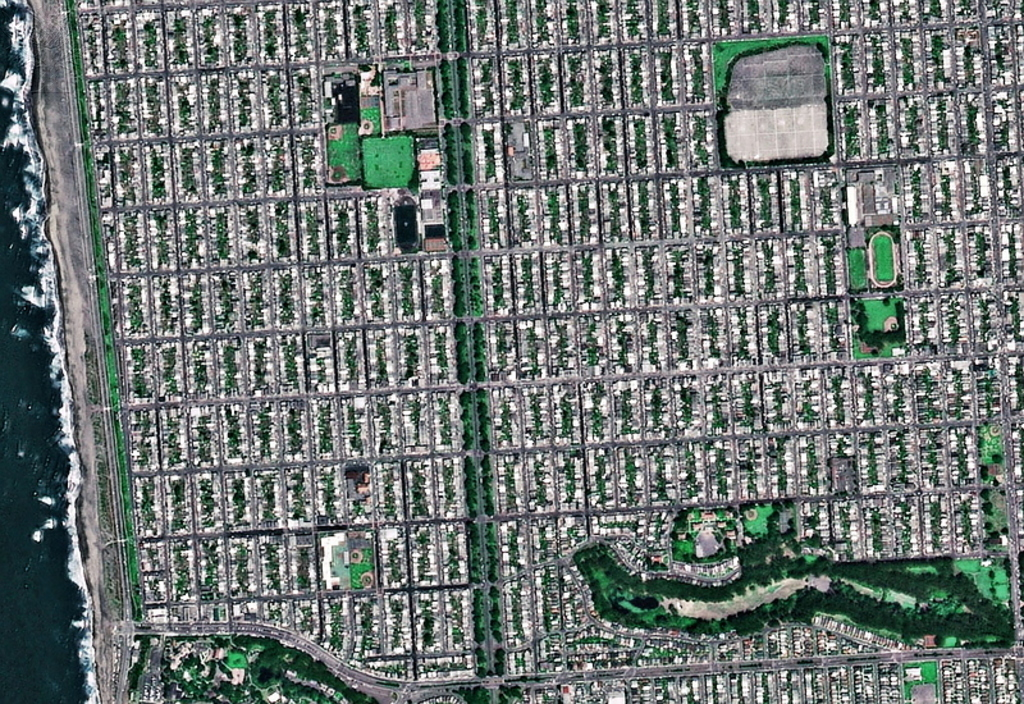
\includegraphics[width=1\linewidth]{Planning report/images/grid_pattern.jpg}
  \caption{Gridiron}
  \label{fig:street_pattern}
\end{subfigure}
~
\begin{subfigure}{.4\linewidth}
  \centering
  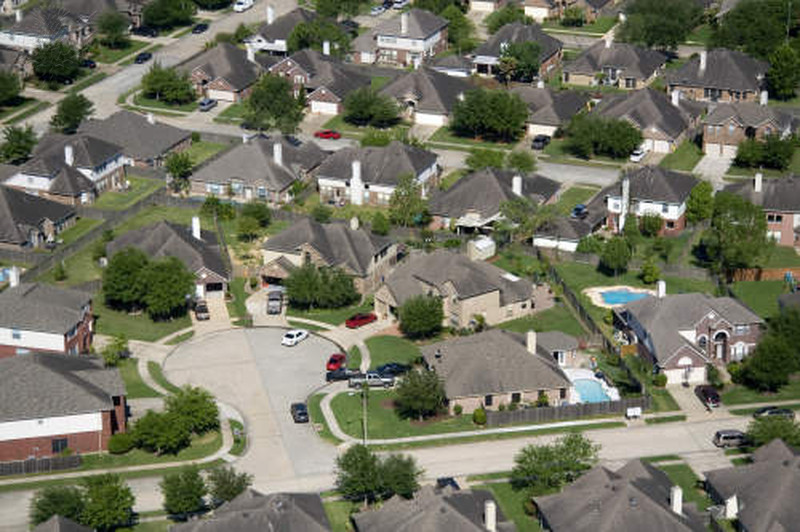
\includegraphics[width=1\linewidth]{Planning report/images/culdesac.jpg}
  \caption{Cul-de-sac}
\end{subfigure}
\caption{Street patterns}
\label{fig:both_pattern}
\end{figure}

\subsection{Unity Editor Scripting}
Creating extensions to the Unity editor can be done with editor scripting. Some examples of what can be added to the workflow are custom windows, menu controls of different kinds. New functionality can also be added to the scene view \cite{unity-extending-editor}. There is an official Unity API for editor scripting which is well documented by Unity Technologies \cite{unity-editor-docs}.
\newpage
\section{Ethics}

The developed tool will probably not affect society in a particular negative way. The only topic worth mentioning is that some people might lose their jobs if companies start using this tool. For instance, people working with designing game cities may be affected, since the tool will automate their jobs. On the other hand, our tool will make game development easier for smaller development teams as well as for hobbyists. Besides, automated generation has been widespread in graphics for decades, and this tool is merely meant to serve as a basis upon which games can be developed.

Since the generated content does not focus on realistically representing the real world, it will disregard some real ethical aspects. It will, for instance, not focus on the ethics of available transportation systems, such as trains and busses, that otherwise are considered in real cities. The tool will instead generate cities that only contain roads used by cars in and around it. This may be seen as only representing a sub-part of the real world, however as described in section \ref{section:delimitations}, the tool focuses on credibility rather than realism.
\newpage
\section{Timetable}
\label{section:timetable}
In figure \ref{fig:timetable}, the preliminary time frame of this project is displayed. The project is mainly scheduled on a weekly basis, with week 1 starting February 3rd. As described in section \ref{section:methodology}, the project is also partitioned into sprints according to the scrum methodology, with the first sprint starting on project week 3. As each sprint is planned on the basis of the current state of the project, the user stories and tasks of the sprints are not marked in the timetable.

Scheduled deadlines are for each row marked with their specified due date within the week of the deadline. Non-dated milestones are implicitly due at the end of their respective week or sprint, and marked as the far right of the boxes of each row. The progress of the thesis is partitioned into three iterations, a first and second draft, as well as the final edit. Likewise, the progress of the developed platform is also partitioned into three iterations, resulting a first and second prototype before the final product. 

\begin{figure}[H]
    \centering
    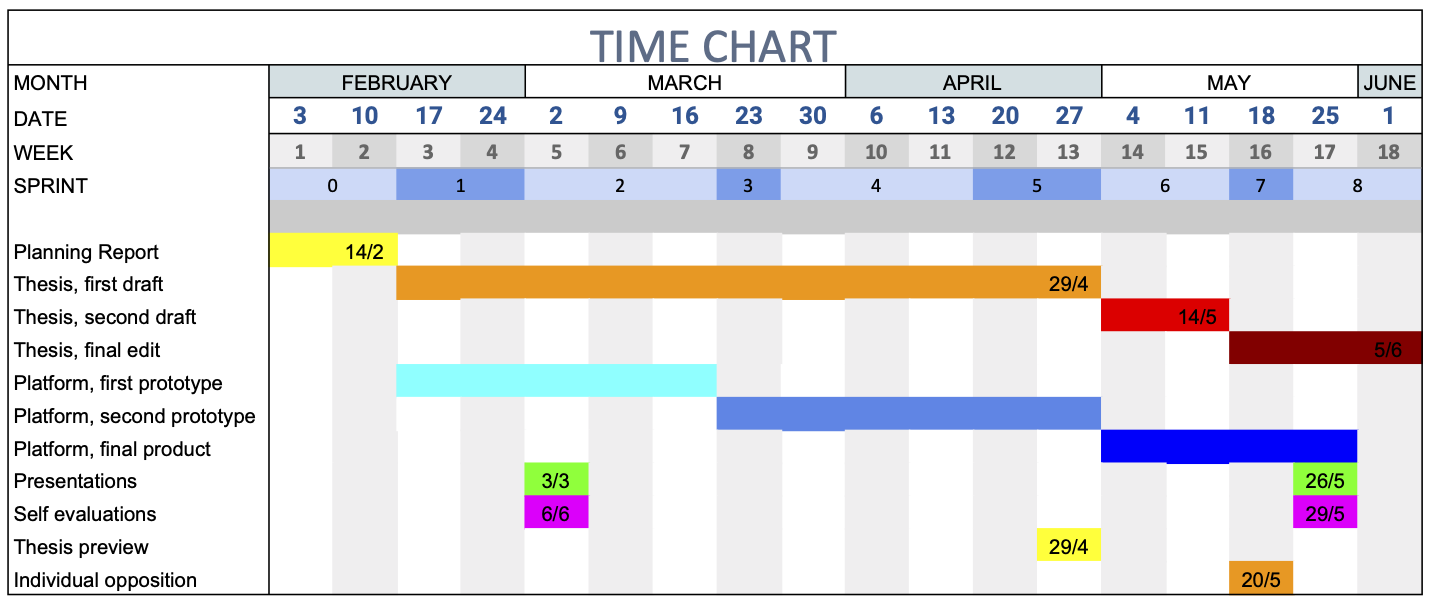
\includegraphics[width = \textwidth]{Planning report/images/timetable.png}
    \caption{The preliminary timetable of the thesis project.}
    \label{fig:timetable}
\end{figure}
\newpage
\addcontentsline{toc}{section}{References}
\printbibliography

\end{document}

% ---- Föreläsning om planeringsrapport ---
% ska finnas på canvas
% specifikt: mål/syfte/metod/plan
% håll fast vid givet upplägg
% problemavsnitt och metod ska vara välskrivna
% titta inte på tidigare planeringsrapporter
% skriv revisionsversion för varje "större" ändring. Visa på varje sida (tror jag att ha sade)
% strikt formel slutrapport

% Bakgrund:
% Viktigt - varför/hur/för vem relevant + vad ska åstakommas

% Syfte:
% Vilka konkreta resultat som ska förmedladas. Relativt kort. 

% Problem / Uppgift:
% Vilka frågor ska besvaras

% Avgränsningar:
% Antingen efter syfte eller i efter slutsats, optimalt med båda.

% Metod / genomförande:
% Testa tankar, iterativt, uppdatera efter hand

% Samhälliga och etiska aspekter
% Ifall det inte finns tydliga etiska aspekter. Motivera varför det inte finns

% Tidsplan
% Konkret. I detalj närmaste tiden och i grova drag längre fram. 
% Milstolpar. 
% Sammanfatta i ett Gantt-schema. 